\subsection{Aricolo: L'istogramma}\label{istogramma}
In questa analisi viene preso come riferimento la pagina: \\
\begin{small}
\url{http://www.fotocomefare.com/istogramma-esposizione-corretta/}.
\end{small}
\\
La struttura di questa pagina è analoga a molte altre pagine del sito, di conseguenza le seguenti osservazioni valgono anche per le altre pagine del sito.\\
Questa pagina soffre di due problemi principali, entrambi legati allo scroll:
\begin{itemize}
\item \textbf{Troppe immagini prima del contenuto}: tra le varie pubblicità, l'immagine introduttiva e le informazioni riguardo l'autore e le condivisioni social, rimane poco spazio per il contenuto e l'utente si trova costretto ad effettuare uno scroll della pagina per visualizzare il contenuto\footnote{Anche con uno schermo con risoluzione 1920x1080 la parte dell'articolo leggibile senza effettuare uno scroll risulta minima};
\item \textbf{La barra laterale}: è presente una barra laterale con i link agli articoli recenti o più visualizzati, questa barra ha una sua scroll bar interna che certe volte porta l'utente a scrollare a vuoto, dato che scrolla il contenuto della barra e non la pagina. Inoltre, come se non bastasse, questa barra è fissa e segue lo scroll della pagina.
\end{itemize}

\begin{figure}[htpb]
\begin{center}
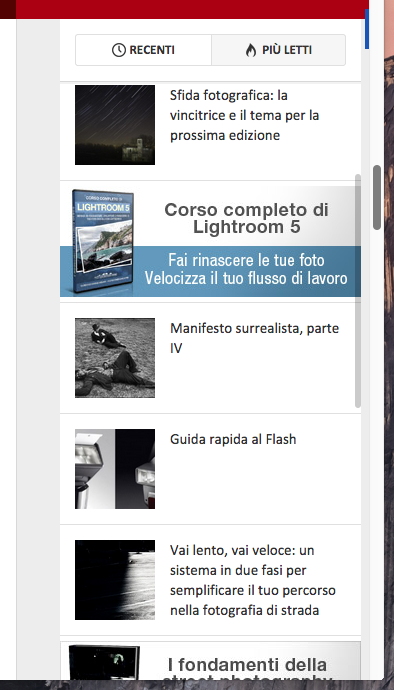
\includegraphics[width=0.6\textwidth]{immagini/barraLaterale.png}
\caption{Barra presente a lato di un articolo, dall'immagine si possono notare le due scroll bar}
\label{barraLaterale}
\end{center}
\end{figure}
\FloatBarrier

Per quanto riguarda il resto della pagina, valgono le stesse osservazioni fatte nella sezione \ref{considerazioniGenerali}.